\documentclass[11pt]{article}
\usepackage[a4paper, total={5in, 8in}]{geometry}
\setlength{\parindent}{0em}
\usepackage{array,booktabs}
\setlength{\parskip}{1em}
\usepackage[utf8]{inputenc}
\usepackage{natbib}
\usepackage{graphicx}
\graphicspath{ {Images} }
\usepackage{enumerate}
\usepackage{url}
\usepackage{tabularx}
\usepackage[table,xcdraw]{xcolor}
\usepackage{hyperref}
\usepackage{algorithmic}
\usepackage{tikz}
\usepackage{caption}
\usepackage{subcaption}
%\usepackage{graphicx}
\usepackage{float}
\usepackage{fancyhdr}

\hypersetup{
    colorlinks,
    citecolor=black,
    filecolor=black,
    linkcolor=black,
    urlcolor=black
}

\usepackage{listings}

\pagenumbering{arabic}

\lstdefinelanguage{CSharp}
{
sensitive=true,
morekeywords=[1]{
abstract, as, base, break, case,
catch, checked, class, const, continue,
default, delegate, do, else, enum,
event, explicit, extern, false,
finally, fixed, for, foreach, goto, if,
implicit, in, interface, internal, is,
lock, namespace, new, null, operator,
out, override, params, private,
protected, public, readonly, ref,
return, sealed, sizeof, stackalloc,
static, struct, switch, this, throw,
true, try, typeof, unchecked, unsafe,
using, virtual, volatile, while, bool,
byte, char, decimal, double, float,
int, lock, object, sbyte, short, string,
uint, ulong, ushort, void},
morecomment=[l]{//},
morecomment=[s]{/*}{*/},
morecomment=[l][keywordstyle4]{\#},
morestring=[b]",
morestring=[b]',
}

\lstset{
backgroundcolor=\color[rgb]{0.95, 0.95, 0.95},
tabsize=2,
rulecolor=,
basicstyle=\scriptsize,
upquote=true,
aboveskip={1.5\baselineskip},
columns=fixed,
showstringspaces=false,
extendedchars=true,
breaklines=true,
prebreak = \raisebox{0ex}[0ex][0ex]{\ensuremath{\hookleftarrow}},
frame=single,
showtabs=false,
showspaces=false,
showstringspaces=false,
identifierstyle=\ttfamily,
keywordstyle=\color[rgb]{1.0,0,0},
keywordstyle=[1]\color[rgb]{0,0,0.75},
keywordstyle=[2]\color[rgb]{0.5,0.0,0.0},
keywordstyle=[3]\color[rgb]{0.127,0.427,0.514},
keywordstyle=[4]\color[rgb]{0.4,0.4,0.4},
commentstyle=\color[rgb]{0.133,0.545,0.133},
stringstyle=\color[rgb]{0.639,0.082,0.082},
}

\makeatletter
\newcount\dirtree@lvl
\newcount\dirtree@plvl
\newcount\dirtree@clvl
\def\dirtree@growth{%
  \ifnum\tikznumberofcurrentchild=1\relax
  \global\advance\dirtree@plvl by 1
  \expandafter\xdef\csname dirtree@p@\the\dirtree@plvl\endcsname{\the\dirtree@lvl}
  \fi
  \global\advance\dirtree@lvl by 1\relax
  \dirtree@clvl=\dirtree@lvl
  \advance\dirtree@clvl by -\csname dirtree@p@\the\dirtree@plvl\endcsname
  \pgf@xa=1cm\relax
  \pgf@ya=-1cm\relax
  \pgf@ya=\dirtree@clvl\pgf@ya
  \pgftransformshift{\pgfqpoint{\the\pgf@xa}{\the\pgf@ya}}%
  \ifnum\tikznumberofcurrentchild=\tikznumberofchildren
  \global\advance\dirtree@plvl by -1
  \fi
}

\tikzset{
  dirtree/.style={
    growth function=\dirtree@growth,
    every node/.style={anchor=north},
    every child node/.style={anchor=west},
    edge from parent path={(\tikzparentnode\tikzparentanchor) |- (\tikzchildnode\tikzchildanchor)}
  }
}

\lstset{language=C}

\pdfpkmode{dpdfezzz}
\pdfpkresolution=8000
\bibliographystyle{unsrt}

%\renewcommand{\contentsname}{Indholdsfortegnelse}
%\renewcommand{\refname}{Litteraturliste}

%\end{document}
% package inclusion and set up of the document
% see, e.g., http://en.wikibooks.org/wiki/LaTeX/Formatting#Hyphenation
% for more information on word hyphenation
\hyphenation{ex-am-ple hy-phen-a-tion short}
\hyphenation{long la-tex}
% 
% see, e.g., http://en.wikibooks.org/wiki/LaTeX/Customizing_LaTeX#New_commands
% for more information on how to create macros

%%%%%%%%%%%%%%%%%%%%%%%%%%%%%%%%%%%%%%%%%%%%%%%%
% Macros for the titlepage
%%%%%%%%%%%%%%%%%%%%%%%%%%%%%%%%%%%%%%%%%%%%%%%%
%Creates the aau titlepage
\newcommand{\aautitlepage}[3]{%
  {
    %set up various length
    \ifx\titlepageleftcolumnwidth\undefined
      \newlength{\titlepageleftcolumnwidth}
      \newlength{\titlepagerightcolumnwidth}
    \fi
    \setlength{\titlepageleftcolumnwidth}{0.5\textwidth-\tabcolsep}
    \setlength{\titlepagerightcolumnwidth}{\textwidth-2\tabcolsep-\titlepageleftcolumnwidth}
    %create title page
    \thispagestyle{empty}
    \noindent%
    \begin{tabular}{@{}ll@{}}
      \parbox{\titlepageleftcolumnwidth}{
        \iflanguage{danish}{%
          
\includegraphics[width=\titlepageleftcolumnwidth]{figures/aau_logo_da}
        }{%
          
\includegraphics[width=\titlepageleftcolumnwidth]{figures/aau_logo_en}
        }
      } &
      \parbox{\titlepagerightcolumnwidth}{\raggedleft\sf\small
        #2
      }\bigskip\\
       #1 &
      \parbox[t]{\titlepagerightcolumnwidth}{%
      \textbf{Synopsis:}\bigskip\par
        \fbox{\parbox{\titlepagerightcolumnwidth-2\fboxsep-2\fboxrule}{%
          #3
        }}
      }\\
    \end{tabular}
    \vfill
    \iflanguage{danish}{%
      \noindent{\footnotesize\emph{Rapportens indhold er frit tilgængeligt, men offentliggørelse (med kildeangivelse) må kun ske efter aftale med forfatterne.}}
    }{%
      \noindent{\footnotesize\emph{The content of this report is freely available, but publication (with reference) may only be pursued due to agreement with the author.}}
    }
    \clearpage
  }
}

%Create english project info
\newcommand{\englishprojectinfo}[8]{%
  \parbox[t]{\titlepageleftcolumnwidth}{
    \textbf{Title:}\\ #1\bigskip\par
    \textbf{Theme:}\\ #2\bigskip\par
    \textbf{Project Period:}\\ #3\bigskip\par
    \textbf{Project Group:}\\ #4\bigskip\par
    \textbf{Participant(s):}\\ #5\bigskip\par
    \textbf{Supervisor(s):}\\ #6\bigskip\par
    \textbf{Copies:} #7\bigskip\par
    \textbf{Page Numbers:} \pageref{LastPage}\bigskip\par
    \textbf{Date of Completion:}\\ #8
  }
}

%Create danish project info
\newcommand{\danishprojectinfo}[8]{%
  \parbox[t]{\titlepageleftcolumnwidth}{
    \textbf{Titel:}\\ #1\bigskip\par
    \textbf{Tema:}\\ #2\bigskip\par
    \textbf{Projektperiode:}\\ #3\bigskip\par
    \textbf{Projektgruppe:}\\ #4\bigskip\par
    \textbf{Deltagere:}\\ #5\bigskip\par
    \textbf{Vejleder:}\\ #6\bigskip\par
    \textbf{Oplagstal:} #7\bigskip\par
    \textbf{Sidetal:} \pageref{LastPage}\bigskip\par
    \textbf{Afleveringsdato:}\\ #8
  }
}

%%%%%%%%%%%%%%%%%%%%%%%%%%%%%%%%%%%%%%%%%%%%%%%%
% An example environment
%%%%%%%%%%%%%%%%%%%%%%%%%%%%%%%%%%%%%%%%%%%%%%%%
\theoremheaderfont{\normalfont\bfseries}
\theorembodyfont{\normalfont}
\theoremstyle{break}
\def\theoremframecommand{{\color{aaublue!50}\vrule width 5pt \hspace{5pt}}}
\newshadedtheorem{exa}{Example}[chapter]
\newenvironment{example}[1]{%
		\begin{exa}[#1]
}{%
		\end{exa}
}
% my new macros
\begin{document}
% Sætter vores listing environment til C# kode ordentligt op.
\lstset {basicstyle=\tiny, tabsize = 2, xleftmargin = 5pt, keepspaces = true, numbersep = 5pt }
%frontmatter
\pagestyle{empty} %disable headers and footers
\pagenumbering{roman} %use roman page numbering in the frontmatter
\pdfbookmark[0]{Forside}{label:frontpage}%
\begin{titlepage}
  \addtolength{\hoffset}{0.5\evensidemargin-0.5\oddsidemargin} %set equal margins on the frontpage - remove this line if you want default margins
  \noindent%
  \begin{tabular}{@{}p{\textwidth}@{}}
    \toprule[2pt]
    \midrule
    \vspace{0.2cm}
    \begin{center}
    \Huge{\textbf{
      Rapport for P3% insert your title here
    }}
    \end{center}
    \begin{center}
      \Large{
        - BuisnessPlanner -% insert your subtitle here
      }
    \end{center}
    \vspace{0.2cm}\\
    \midrule
    \toprule[2pt]
  \end{tabular}
  \vspace{4 cm}
  \begin{center}
    {\large
      Projektrapport 3. semester%Insert document type (e.g., Project Report)
    }\\
    \vspace{0.2cm}
    {\Large
      Gruppe ds315e15%Insert your group name or real names here
    }
  \end{center}
  \vfill
  \begin{center}
  Aalborg Universitetet\\
  Datalogi
  \end{center}
\end{titlepage}
\clearpage

\thispagestyle{empty}
{\small
\strut\vfill % push the content to the bottom of the page
\noindent Copyright \copyright{} Aalborg University 2015\par
\vspace{0.2cm}
\noindent Skrevet i \LaTeX ud fra template lavet af Jesper Kjær Nielsen. 
}
\clearpage


%\pdfbookmark[0]{English title page}{label:titlepage_en}
%\aautitlepage{%
%  \englishprojectinfo{
%    Project Title %title
%  }{%
%    Scientific Theme %theme
%  }{%
%    Fall Semester 2010 %project period
%  }{%
%    XXX % project group
%  }{%
%    %list of group members
%    Author 1\\ 
%    Author 2\\
%    Author 3
%  }{%
%    %list of supervisors
%    Supervisor 1\\
%    Supervisor 2
%  }{%
%    1 % number of printed copies
%  }{%
%    \today % date of completion
%  }%
%}{%department and address
%  \textbf{Electronics and IT}\\
%  Aalborg University\\
%  \href{http://www.aau.dk}{http://www.aau.dk}
%}{% the abstract
%  Here is the abstract
%}

\cleardoublepage
{\selectlanguage{danish}
\pdfbookmark[0]{Titelblad}{label:titlepage_da}
\aautitlepage{%
  \danishprojectinfo{
    P3 rapport %title
  }{%
    Udvikling af applikationer – fra brugere til data, algoritmer og test – og tilbage igen %theme
  }{%
    Efterårssemesteret 2015 %project period
  }{%
    ds315e15 % project group
  }{%
    %list of group members
    Charlie Dittfeldt Byrdam\\
    Jesper Windelborg Nielsen\\    
    David Jahanshiri\\
    Nicklas Embo\\
    Rasmus Nørskov\\
    Mark Lauridsen\\
    Andreas Sommerset
  }{%
    %list of supervisors
    Dalia Kaulakiene\\
  }{%
    10 % number of printed copies
  }{%
    27-05-2055 % date of completion
  }%
}{%department and address
  \textbf{Datalogi}\\
  Aalborg Universitet\\
  \href{http://www.aau.dk}{http://www.aau.dk}
}{% the abstract
Abstract, bla bla bla
}}

\clearpage

\vspace{\baselineskip}\hfill Aalborg University, d. 27 maj 2015
\vfill\noindent
\begin{minipage}[b]{0.45\textwidth}
 \centering
 \rule{\textwidth}{0.5pt}\\
  Charlie Dittfeldt Byrdam\\
 {\footnotesize <cbyrda14@student.aau.dk>}
\end{minipage}
\hfill
\vspace{3\baselineskip}
\begin{minipage}[b]{0.45\textwidth}
 \centering
 \rule{\textwidth}{0.5pt}\\
  Jesper Windelborg Nielsen\\
 {\footnotesize <jwni14@student.aau.dk>}
\end{minipage}
\hfill
\vspace{3\baselineskip}
\begin{center}
\begin{minipage}[b]{0.45\textwidth}
 \centering
 \rule{\textwidth}{0.5pt}
  John Doe\\
 {\footnotesize <johndoe@student.aau.dk>}
\end{minipage}
\end{center}
\cleardoublepage%
\pdfbookmark[0]{Table of Contents}{label:contents}
\pagestyle{fancy} %enable headers and footers again
\tableofcontents
\chapter*{Preface\markboth{Preface}{Preface}}\label{ch:preface}
\addcontentsline{toc}{chapter}{Preface}

This report is written by group ds315e15, fall 2015.

For citations we use the "Vancouver Numeric" method, where citations have this form: \textit{Test citation 1}[1]. This means that further information about "Test Citation 1", is found as [1] in the "References" section of this report.

Citations have the following parameters: \textit{author, title, publishing method, year, online-status, last visited}. \newline

The finished product -???????- is a program written in the programming language C\#. Because the report uses technical terminology, it is recommended that the reader have some knowledge of C\# or a similar object-oriented programming language.

%\noindent Det færdige produkt for denne rapport kaldes CAS.NET. Kildekoden til CAS.NET og rapporten som PDF kan findes på den vedlagte disk.
%\noindent The finished product for this is called ?????????. The source code 
\cleardoublepage
%mainmatter
\pagenumbering{arabic} %use arabic page numbering in the mainmatter
\chapter{Introduction}\label{ch:Indledning}
Dette er den super gode indledning.\cite{website:Eksempel}

\section{Initial Problem}
When starting a new company, a big concern is how you will manage your business. 
According to Lawyer Dorte Kjærgaard, who has worked with many startups, this can often be a challenge. There are many different tasks when running a company. Often times many different IT systems are needed in order to keep track of customers, expenses, projects, products and more. This complicates support and makes it harder to integrate new team members in the workflow.
A system that integrates these different processes into a single product, would streamline the business management pipeline. 
%Rather than many different tools a single 

\textbf{How can an IT system, that can help startups manage their business, be constructed?}
\chapter{Documentation}\label{ch:Documentation}

\input{sections/methods.tex}
\section{Systemselection}
\section{Problem Domain}

This chapter will analyze different aspects of the problem domain for our solution. The purpose of this is to produce a complete model of the problem domain, from which will answer the question: \textit{What data will the system process?}. 
We will accomplish this by looking at classes, structures and actions relevant to our system definition. \\
Our methods of analysis are borrowed from the book "Objected-oriented Design"\citep{FACTORPage}. It is recommended, although not necessary, to have knowledge of the methods used in the book. %In the following chapters we will refer to the program that we aim to make as our "solution".

The analysis of the problem domain consists of three points:
\begin{itemize}
\item \textbf{Classes:} Describes the system's classes.
\item \textbf{Events:} Lists events relating to the classes, resulting in a  
\item \textbf{Structure:} Describes the relationships between classes and objects, resulting in a class diagram.
\item \textbf{Behavior:} Describes the objects' behavior and interaction, and results in state diagrams.
\end{itemize}

By analyzing these different points of interest, insight is gained into which objects are relevant, what relations there are between them as well as their behavior.
With this insight it is easier to gauge how the system should be built, in order to handle the objects from the problem domain.

\subsection{Classes}

The problem domain can be described in terms of classes. Classes are the primary building blocks used to define and outline the problem domain. 

Through the process of brainstorming, we have been able to produce a list of classes that would be a good fit for the data that we would store.

The classes have been divided into four different groups, one group for each part of the program, as described in our system definition.

\subsubsection*{Main}
This is the main section of the program. When the user logs in to the program, they see information about their company. The main menu provides a variety of options, used to manage the company, and the projects it is currently working on. From this page it is also possible to view the company's employees and customers, along with additional information about them.

\begin{itemize}
  \item \textbf{Company} \\
 The company class is one of the main classes in the program. It will be used to keep track of the data of a specific company. A company can be created by a user and has users associated with it.
  
%This is the main module in the program. A company page is the hub for which all the information about the company is contained. It is possible to access multiple modules from this module. information such as VAT identification number (VATIN), clients and employees.
  
 % \item \textbf{Project Management} 
  
%When a company wants to produce something, or provide a service, they create a project for the company. This is done in the project management module. From here it is possible to assign employees to different projects, in different roles. From the project management page, you can choose from the different projects the company currently is working on, and view information about them. Each project has a separate budget, set by the project admin. This budget is used on salaries and product creation.
  
   information. 
  \item \textbf{User} \\
The user class identifies the users of the program. A user class can create or join companies, and its association with the company class, show its current status in a specific company, such as employer or employee.
  
%Contains information about the employees in a company. Information such as the employees names, rank and current projects.
\end{itemize}

\subsubsection*{CRM}

\begin{itemize}
  %\item \textbf{Documents} Information like document name, location, context etc.
  
  \item \textbf{Customer} \\
  The user class identifies the customers. It has attributes such as name, contact info. It is associated with the company class.
\end{itemize}

\subsubsection*{Project}

\begin{itemize}
  \item \textbf{Project} \\
This class contains information about projects, with attributes such as project name and users connected to the project. It is associated with both the user, company and customer classes.
  \item \textbf{Task} \\
Information about tasks that are connected to individual projects. Attributes such as name, description, employee(s) assigned, deadline.
  \item \textbf{Task Comment} \\
Users can comment on an existing task. that are connected to individual projects. Attributes like comment content and employee.

\end{itemize}



\subsubsection*{Finance}

\begin{itemize}
  \item \textbf{Budget} \\
  This class contains finance information, such as expenditure and income. 
  % Taxes, capital, profit reinvestment.
 
  %\item \textbf{Income} Information such as, name, company, time etc.

\end{itemize}

\subsection{Events}
From the classes, we have below derived a number of events that could take place between objects from the different classes. Identifying these events is important, as it improves our knowledge of what needs to be implemented in the program.

To create an overview of the events and the connection between events and classes, we have created an event table. By looking at the event table you can quickly see what events are related to which classes.
That there is a symbol indicates, a relation between an event and a class. The "+" symbol indicates that the event can happen 0 and 1 times for each object and the "*" symbol indicates that the event can happen 0 or more times.


\hspace*{-2,5cm}
\begin{tabular}{|l||c|c|c|c|c|c|c|c|}
  \hline
                                   & Company & Employee & Project & Customer & Budget  & Product & Task    & TC*             \\\hline \hline
   Customer added                  &    *    &          &         &     +    &         &         &         &                 \\\hline
   Customer updated                &    *    &          &         &     *    &         &         &         &                 \\\hline 
   Customer deleted                &    *    &          &         &     +    &         &         &         &                 \\\hline
   Project added                   &    *    &    *     &    +    &     *    &         &         &         &                 \\\hline
   Project updated                 &         &    *     &    *    &          &         &         &         &                 \\\hline
   Project deleted                 &    *    &    *     &    +    &     *    &         &         &         &                 \\\hline
   Task added                      &         &          &    +    &          &         &         &   +     &   *             \\\hline 
   Task deleted                    &         &          &    *    &          &         &         &   +     &   +             \\\hline
   Task updated                    &         &    *     &    *    &          &         &         &   *     &   *             \\\hline
   Task finished                   &         &    *     &    *    &          &         &         &   +     &   +             \\\hline
   TC added                        &         &    *     &         &          &         &         &   *     &   *             \\\hline
   TC updated                      &         &    *     &         &          &         &         &   *     &   *             \\\hline
   TC deleted                      &         &    *     &         &          &         &         &   *     &   *             \\\hline
   Product added                   &    *    &          &         &          &         &    +    &         &                 \\\hline
   Product deleted                 &    *    &          &         &          &         &    +    &         &                 \\\hline
   Product updated                 &    *    &          &         &          &         &    *    &         &                 \\\hline
   Income added                    &    *    &          &         &     *    &    +    &         &         &                 \\\hline
   Income updated                  &    *    &          &         &     *    &    *    &         &         &                 \\\hline
   Expense added                   &    *    &          &         &     *    &    +    &    *    &         &                 \\\hline
   Expense updated                 &    *    &          &         &     *    &    *    &         &         &                 \\\hline
   Employee added                  &    *    &    +     &         &          &         &         &         &                 \\\hline
   Employee updated                &    *    &    *     &         &          &         &         &         &                 \\\hline
   Company added                   &    +    &          &         &          &         &         &         &                 \\\hline
   Company updated                 &    *    &          &         &          &         &         &         &                 \\
  \hline
\end{tabular}
\textit{* TC stands for Task Comment}
                                                                                                                                 
Based on the event table, each class has an adequate amount of events attached. Since the events are spread out over the classes, it means that there is no one class that has too many events compared to the other classes. %Had there been a class with too many events, we should have considered if it could be divided into several classes. 

\subsection{Structure}
To describe the relations between the different classes, a class diagram has been created.

\begin{figure}[H]
    \centering
    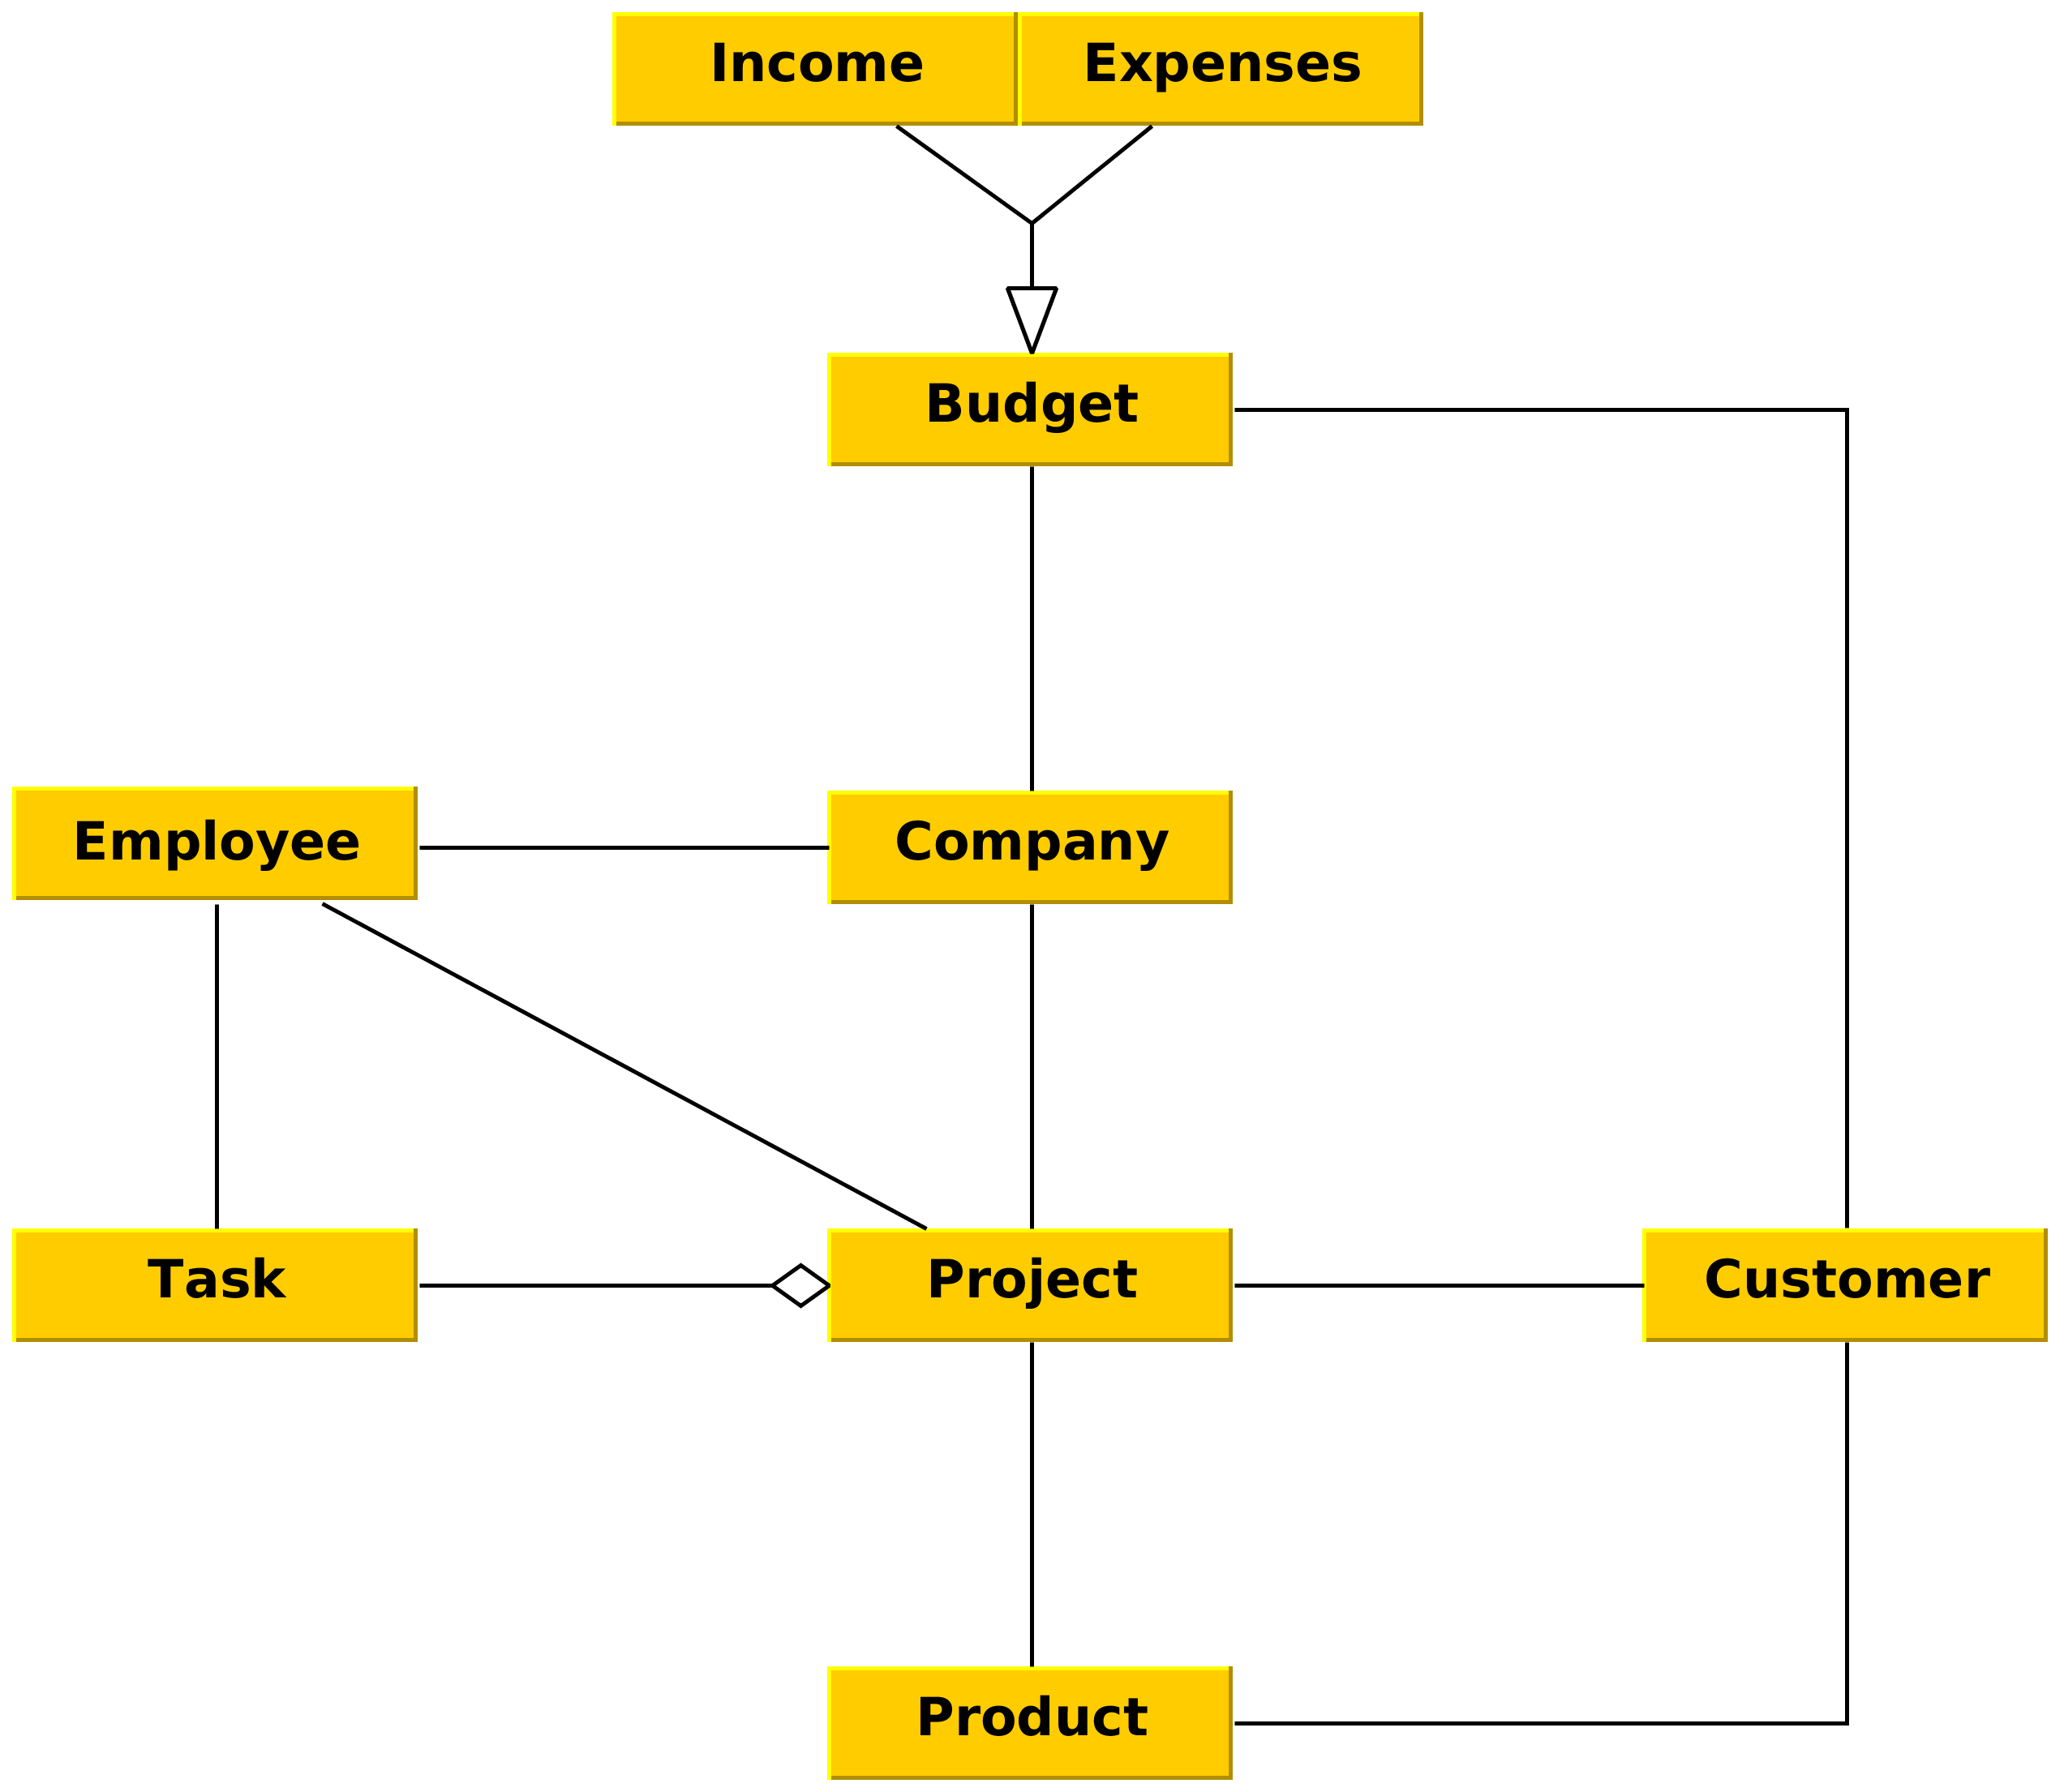
\includegraphics[scale=0.12]{Images/ProblemDomain/klassediagram.png}
    \caption{Class Diagram ???????}
    \label{fig:Class Diagram}
\end{figure}

\subsection{Behavior}

Based on the events in the event table, we can make behavioral patterns. The overall behavior of different objects is made up of the order in which events are run (event traces) and the behavioral patterns of the given object. %An event trace, a sequence of events, describes in which order different events can be run for a given object. 
\\
Behavioral patterns can be described by statechart diagrams. State diagrams give an abstract description of system behavior, by taking an object of a single class and showing the different states it will inhabit as it goes through the system.
We have therefore made statechart diagrams of some of the more important events. These statechart diagrams will be based on the events we uncovered in the event table.



\paragraph{Company}

\begin{figure}[H]
    \centering
    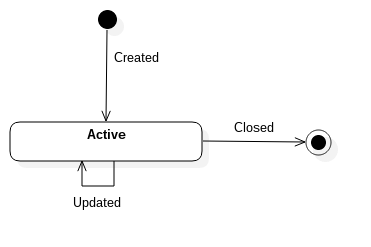
\includegraphics[scale=0.7]{Images/ProblemDomain/companyActivityDiagram.png}
    \caption{Company Activity}
    \label{fig:companyActivityDiagram}
\end{figure}

\paragraph{Customer}

\begin{figure}[H]
    \centering
    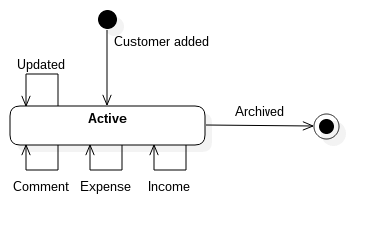
\includegraphics[scale=0.7]{Images/ProblemDomain/customerActivityDiagram.png}
    \caption{Customer Activity}
    \label{fig:customerActivityDiagram}
\end{figure}

\paragraph{Employee}

\begin{figure}[H]
    \centering
    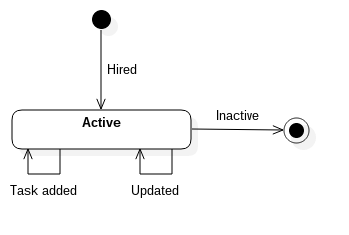
\includegraphics[scale=0.7]{Images/ProblemDomain/employeeActivityDiagram.png}
    \caption{Employee Activity}
    \label{fig:employeeActivityDiagram}
\end{figure}

\paragraph{Project}

\begin{figure}[H]
    \centering
    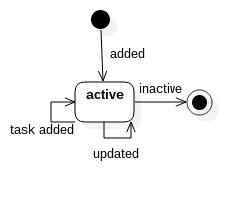
\includegraphics[scale=0.7]{Images/ProblemDomain/projectActivityDiagram.png}
    \caption{Project Activity}
    \label{fig:projectActivityDiagram}
\end{figure}

\paragraph{Product}

\begin{figure}[H]
    \centering
    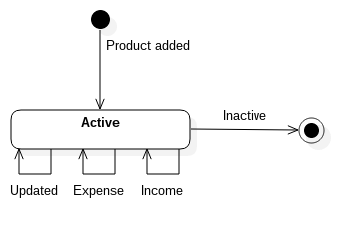
\includegraphics[scale=0.7]{Images/ProblemDomain/productActivityDiagram.png}
    \caption{Project Acitivty}
    \label{fig:productAcitvityDiagram}
\end{figure}

\paragraph{Task}

\begin{figure}[H]
    \centering
    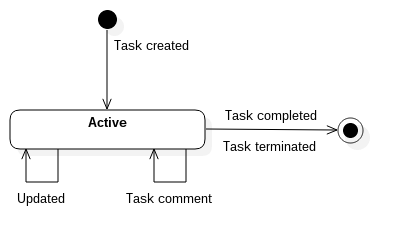
\includegraphics[scale=0.7]{Images/ProblemDomain/taskActivityDiagram.png}
    \caption{Task Activity}
    \label{fig:taskActivityDiagram}
\end{figure}

\paragraph{Task comment}

\begin{figure}[H]
    \centering
    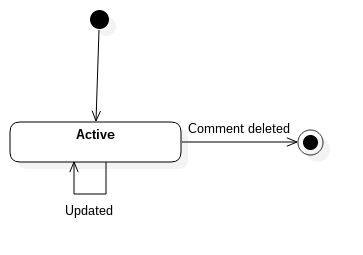
\includegraphics[scale=0.7]{Images/ProblemDomain/tcActivityDiagram.png}
    \caption{Task comment Activity}
    \label{fig:tcActivityDiagram}
\end{figure}

\paragraph{Budget}

\begin{figure}[H]
    \centering
    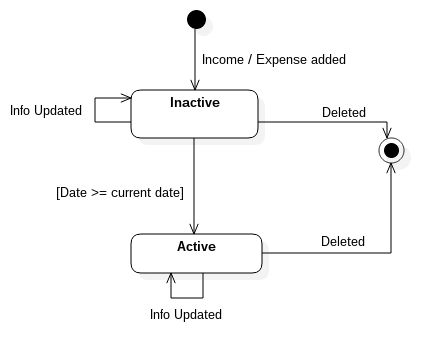
\includegraphics[scale=0.7]{Images/ProblemDomain/budgetActivityDiagram.png}
    \caption{Budget Activity}
    \label{fig:budgetActivityDiagram}
\end{figure}
















\subsection{Summary}

In this chapter the different classes relevant to the problem domain have been found. Events have been found for each of these classes. 
Based on those events a class diagram has been produced, demonstrating the relations between the different classes. Furthermore the behavior of a number of important classes has been analyzed. Based on all this is now a foundation for what classes the final program should contain, their relations and their behavior.

The next chapter will focus on the context in which the solution would be used. The chapter take a closer look at what the solution should be able to do, how users will be using the solution and to best make the solution fit the needs of the users.















\section{Application Domain}

In this chapter the application domain will be studied, with the aim of gaining a better insight into the context in which the solution should be implemented.

The methods of analysis used are borrowed from the book "Objected-oriented Design"\citep{FACTORPage}. It is recommended, although not necessary, to have knowledge of the methods used in the book.

The application domain is defined as the organization that manages, monitors, or controls a problem domain.

From our analysis of the application domain, this section should aim to answer the question:
\begin{itemize}
    \item How should the IT system be used?
\end{itemize}


The purpose of the analysis is to determine the requirements for using the system. This is done by examining these points:
\begin{itemize}
\item \textbf{Use:} Determines how the actors interact with the system and results in a description
of use cases and actors.
\item \textbf{Features:} Provides requirements for information processing in the application domain and performance
provides a complete feature list of specifications of complex functions.
\item \textbf{User interface:} Defines the system's user interface and results in a complete overview of the user interface.
\end{itemize}

Use and functions will provide insight into the actual use of the system and what features are
necessary to solve the issues that exist in the problem domain.
Interface section provides a picture of what the finished system should look like, which can be using during system development.

Once the application domain has been analyzed, there should be specific parts for both functionality and user interface that can be implemented in a solution.

\subsection{Use}
In this section, actors and use cases will be described and investigated. The objective of this part of the analysis, is to get an overview of how users interact with the system and get an overview of the requirements the system must meet.

An actor is a person or an IT program that uses the mentioned system. A specific user can act as several different actors and different users can appear as the same actor. An actor is described by using an actor specification. An actor specification consists of the following:

\begin{itemize}
    \item \textbf{Purpose:} Describes what purpose the actor serves in relation to the system.
    \item \textbf{Characteristics:} Unique characteristics or actions related to the do their job.
    \item \textbf{Example:} Small very generalized scenario describing how this actor could use the system.
\end{itemize}

A use case is an abstraction of the interaction between the actors and the system. It can be described by the use of a use case specification. A use case specification consists of the following items:
\begin{itemize}
    \item \textbf{Use Case:} A description of the system flow for a specific task, what actions you take to get from A to B in the program.
    \item \textbf{Objects:} The objects that are affected by the use case. 
    \item \textbf{Features:} The features that the use case uses. 
\end{itemize}


\subsubsection{Actors}

The following three actors are the basic types of people who will be using the system. \\

\fbox{\begin{minipage}{32.3em}
\textbf{Employee:}
\begin{description}
  \item[Purpose] \hfill \\
  The average employee who works on company projects. Needs be able to access projects he/she is assigned to.
  \item[Characteristics] \hfill \\
  Varying levels of familiarity with the system.
  \item[Example] \hfill \\
  Uses the system many times a day to access her project page, in order to view tasks, create new ones and view overall progress or comments. The system is essential for coordination of the project.
%\ldots
\end{description}
\end{minipage}}

\fbox{\begin{minipage}{32.3em}
\textbf{Super Employee:}
\begin{description}
  \item[Purpose] \hfill \\
  Senior employee who works on company projects. Needs be able to access projects he/she is assigned to and is able to create new projects. Can moderate projects he/she has access to, e.g. delete comments and tasks of others. Has access to CRM system entries related to current projects in order to facilitate contact with the customer.
  \item[Characteristics] \hfill \\
  Senior employee, high level of familiarity with the system.
  \item[Example] \hfill \\
  A:
  Uses the system many times a day to access her project page, in order to view tasks, create new ones and view overall progress or comments. The system is essential for coordination of the project. May access CRM to input new customer data or read existing, in order to contact customer to recieve clarification on requirements.
  B:
  Will use the system to setup a new project page when new projects arise. Will manage them and moderate content within.
%\ldots
\end{description}
\end{minipage}}

\fbox{\begin{minipage}{32.3em}
\textbf{CEO:}
\begin{description}
  \item[Purpose] \hfill \\
  CEO of the company. Has admin access to everything. Needs access to CRM and finance. Depending on size of   company may also participate in projects, but if not will still view projects in order to judge progress.
  \item[Characteristics] \hfill \\
  Depending on the size and structure of a company, the CEO may be more or less hands-on. Will have varying needs and experience.
  \item[Example] \hfill \\
  CEO needs to contact a customer to report on progress and get feedback on some decisions related to a project. The CEO goes to the CRM module to find his/her contact information. The CEO then visits the project page to gauge current progress.
  
\end{description}
\end{minipage}}


\fbox{\begin{minipage}{32.3em}
\textbf{Customer:}
\begin{description}
  \item[Purpose] \hfill \\
  Customer of the company. Needs access read-access to the project that he is currently paying the company to make.
  \item[Characteristics] \hfill \\
  Will have varying levels of experience with technology.
  \item[Example] \hfill \\
  A very hands-on customer who likes to know how the project is progressing, without going through a middle-man.
\end{description}
\end{minipage}}


\subsubsection{Use cases}

Use cases are used to create a better overview of the actors interaction with the system. Use cases are a list of action or event steps, detailing interactions between an actor and a system, with the aim of achieving a goal.
The use cases are presented in the form of text, where a given use case is described. 

\fbox{\begin{minipage}{32.3em}
\textbf{Create New Task:}
\begin{description}
  \item[Actor(s)] \hfill \\
  CEO, Super Employee, Employee
  
  \item[Use Case] \hfill \\
  A new task can be created by any user who has access to the project he wishes to create a new task in. The user enters the project page for the project he wishes to create a new task for. %He is taken to the overview of the project where he can see, statistics, deadlines and other information. 
  He is then taken to the project overview where the user can see an overview of the tasks. The user presses the "Create New Task" button,  where after he is taken to the task creation page. Here the user inputs the relevant data and the system then receives the data, it will give an error message if the input is not accepted. If the input is accepted the use case is ended and a new task is created.
  
  \item[Objects] \hfill \\
  Project, task.

\end{description}
\end{minipage}}

\fbox{\begin{minipage}{32.3em}
\textbf{Add New Task Comment:}
\begin{description}
  \item[Actor(s)] \hfill \\
  CEO, Super Employee, Employee
  \item[Use Case] \hfill \\
   A new comment can be added to a task by any user who has access to the project in which the chosen task resides. The user enters the project page for the project he wishes to create a new task for. %He is taken to the overview of the project where he can see, statistics, deadlines and other information. 
  He is then taken to the project overview where the user can see an overview of the tasks. Clicking on a task will take the user to page containing detailed info of only this task. 
  There will be a text box towards the bottom of the page with a submit below it. The user fills out the text box with their comment, presses the submit button and the system then receives the data. It will give an error message if the input is not accepted. If the input is accepted the use case is ended and a new comment is added to the task.
  
  \item[Objects] \hfill \\
  Project, task, task comment.

\end{description}
\end{minipage}}

\fbox{\begin{minipage}{32.3em}
\textbf{View Project:}
\begin{description}
  \item[Actor(s)] \hfill \\
  CEO, Super Employee
  \item[Use Case] \hfill \\

  \item[Objects] \hfill \\
  Project, User

\end{description}
\end{minipage}}


\fbox{\begin{minipage}{32.3em}
\textbf{Create New Project:}
\begin{description}
  \item[Actor(s)] \hfill \\
  CEO, Super Employee
  \item[Use Case] \hfill \\
 New projects can be created by super employees and CEO's. They will create new projects by first visiting the "Project Overview" menu item. This will bring them to a page where one can see an overview of the projects the user has access to. The user presses the "Create New Project" button,  where after he is taken to the project creation page. Here the user inputs the relevant data and the system then receives the data, it will give an error message if the input is not accepted. If the input is accepted the use case is ended and a new project is created.
  
  \item[Objects] \hfill \\
  Project, User

\end{description}
\end{minipage}}

\fbox{\begin{minipage}{32.3em}
\textbf{Update Project Settings:}
\begin{description}
  \item[Actor(s)] \hfill \\
  CEO, Super Employee   
  \item[Use Case] \hfill \\
 Projects can be edited by super employees and CEO's. CEO's can access all projects, super employees only those they themselves have created. They will edit projects by first visiting the "Project Overview" menu item. This will bring them to a page where one can see an overview of the projects the user has access to. The user clicks on a project, where after he is taken to the detailed information page for the specific project. Here the user can edit existing data or input new relevant data. The system then receives the data, it will give an error message if the input is not accepted. If the input is accepted the use case is ended and the project has been successfully edited.
  
  \item[Objects] \hfill \\
  Project, User

\end{description}
\end{minipage}}

\fbox{\begin{minipage}{32.3em}
\textbf{Create New Expense/Income entry:}
\begin{description}
  \item[Actor(s)] \hfill \\
  CEO
  \item[Use Case] \hfill \\
CEO's can view finance information and add new expenses. First they visit the Finance page where they can see an overview of finances. There will be a menu item called "New", hovering over this will reveal two new menu items, that allow the user to choose between creating a new expense entry or creating a new income entry. Choosing one of these menu items will  bring the user to a new page, where the user inputs the relevant data. The system then receives the data and will give an error message if the input is not accepted. If the input is accepted the use case is ended and a new expense/income entry is created.

  \item[Objects] \hfill \\
  Budget

\end{description}
\end{minipage}}

\fbox{\begin{minipage}{32.3em}
\textbf{Create New Customer entry in CRM system:}
\begin{description}
  \item[Actor(s)] \hfill \\
  CEO, Super Employee
  \item[Use Case] \hfill \\
CEO or super employees can access the CRM system, but only the CEO those assigned to projects him/herself is not currently assigned to. First they visit the CRM page where they can see an overview of customers. The user presses the "Add New Customer" button,  where after he is taken to the customer adding page. Here the user inputs the relevant data and the system then receives the data, it will give an error message if the input is not accepted. If the input is accepted the use case is ended and a new customer is added.
  \item[Objects] \hfill \\
  Customer
\end{description}
\end{minipage}}


\subsection*{Actor Table}
Below is the actor table. The actor table shows the link between actors and the use cases. It gives you an overview of which actors can potentially execute which use cases. Besides the CEO, all the different actors are limited to accessing that which they are entitled to.

\begin{table}[h]
\centering
%\caption{My caption}
\label{my-label}
\begin{tabular}{|
>{\columncolor[HTML]{EFEFEF}}l |c|c|c|c|}
\hline
                   & \multicolumn{1}{l|}{\cellcolor[HTML]{EFEFEF}CEO} & \multicolumn{1}{l|}{\cellcolor[HTML]{EFEFEF}Super Employee} & \multicolumn{1}{l|}{\cellcolor[HTML]{EFEFEF}Employee} & \multicolumn{1}{l|}{\cellcolor[HTML]{EFEFEF}Customer} \\ \hline
View Project       & x                                                & x                                                           & x                                                     & x                                                     \\ \hline
New Task           & x                                                & x                                                           & x                                                     &                                                       \\ \hline
New Task Comment   & x                                                & x                                                           & x                                                     &                                                       \\ \hline
New Project        & x                                                & x                                                           &                                                       &                                                       \\ \hline
Update Project     & x                                                & x                                                           &                                                       &                                                       \\ \hline
New Customer       & x                                                & x                                                           &                                                       &                                                       \\ \hline
New Expense/Income & x                                                &                                                             &                                                       &                                                       \\ \hline
\end{tabular}
\end{table}

The use cases described will be used when planning the user interface for the system. Using the combined info from actors and use cases seen in the actor table, it should be easy to identify what permissions the different user types should have, when developing the system.


\subsection{Functions}

This purpose of this section is to identify all the functions the system should have, in order to then determine the requirements for these functions. Functions are defined as "a facility for making a model useful for actors", they essentially feed a system model with information. 
We will be using the use cases and events from prior sections, to lay the foundation for these functions.

Functions can be classified into different types. There are four different types of functions. The following definitions of the types are taken from the book "Objected-oriented Design"\citep{FACTORPage}.

\begin{itemize}
 
\item Update: Update functions are activated by a problem domain event and result in a change in the model’s state. 

\item Signal: Signal functions are activated by a change in the model’s state and result in a reaction in the context; this reaction can be a display to the actors in the application-domain or a direct intervention in the problem-domain 

\item Read: Read functions are activated by an actor’s need for information and result in the system displaying information about the model. 

\item Compute: Compute functions are activated by a need for information in an actor’s work tasks and consists of a computation involving information provided by the actor and/or the model; the result is a display of the computation’s result. 

\end{itemize}

Functions are not necessarily a single type. Complex functions may be classified as multiple types. \\






\subsection{User Interface}


\section{Requirements specification}
In this section will there be described, that we got from our contact Dorthe Kjærgaard. She sent some documentation for her ideas, about the solution and what is required in the ideal solution. 

\subsection{General requirements}

\subsection{CRM module}

The ideal solution should have a customer relationship management (CRM) module. A CRM module is used to organize and make customer information available in a organized and structured way. The CRM module should contain informations of customers, suppliers, and business contacts, thereby the CRM module should contain more information than just direct customer informations.\\
\\
The CRM module should be able to make some automated tasks such as reminders or automated billing features. It should also make it possible to assign users to a specific project and to see the billing history of the user. At the same time the module should keep a history and be able to log all interactions with the customer. It should also be able to attach files as for example contracts.

\subsection{Project module}
The ideal solution must have a project module. The module must contain general information about the project, such as the title, a description and the employees assigned to the project. The module will have information about the budget for the project, and the project leaders will be able to assign task to the employees under them, will at the same time be able to monitor the progress of the currently active task, and also the monitor the progress of the whole project.

\subsection{Booking system}

\subsection{Employee module}
The ideal solution must contain a employee module. The module will contain different kinds of information about the employee. Some of the information would be recruitment papers which would be papers for getting a job in the organization, papers like recruitment application, the employees CV and education papers would be relevant. \\
Another group of information about the employee will be employment details such as, the employment contract, agreement between both parties and a specific job description would be relevant. The module must also contain some general information about the company and employee relationship, such a employee handbook, a organization diagram and overall job description.

\subsection{Document module}

The ideal solution should contain a document module. The document module should should contain documents relevant for the organization.\\
\\
Relevant documents could be organizational documents like register of owners and deed of organization. It could also contain documents about tax or permits or the register certificate of the organization.\\
\\
The document module could also contain documents for running the company like business plans or organizational diagrams. It could also have documents for tasks like checklists, a design manual or progress descriptions.\\
\\
The document module could contain general contracts, cooperation agreements or business terms.\\
\\
The document module could have financial documents, like annual final report or budget plans.

\subsection{Sales module}
\input{sections/design.tex}
\input{sections/implementation.tex}
\input{sections/test.tex}
\chapter{Konklusion}\label{ch:Konklusion}
Dette er den helt vildt fede konklusion.
\section{Glossary}

Ord og den slags står her
\begin{itemize}
	\item \textbf{CRM} write about me plzzzzzz
\end{itemize}
\bibliography{bib/mybib}\label{bib:mybiblio}
\appendix
\chapter{Appendix a}\label{ch:bilagA}

Næ, her står sku ingenting endnu.
\end{document}
